\ac{ML} is a branch of \ac{AI} that uses algorithms capable of learning from data and generalizing to unseen data to perform specific tasks. Tom Mitchell (1997) proposed an engineering-oriented definition of ML: "\textit{A computer program is said to learn from experience E with respect to some task T and some performance measure P, if its performance on T, as measured by P, improves with experience E}."

\ac{DL} is a subset of ML based on multi-layered neural networks (hence the term \textit{deep}) to model complex patterns in large datasets. DL has demonstrated remarkable success in various fields, such as computer vision and natural language processing, due to its ability to automatically extract relevant features from raw data. 
% Neural networks were inspired from the human brain

The simplest neural network architecture, the perceptron, was invented by Frank Rosenblatt in 1957. It was sufficient for solving linearly separable tasks but limited in handling non-linear problems. Neural networks were subsequently improved to address increasingly complex tasks. Examples of key advancements include:
\begin{itemize}
    \item \textbf{\ac{MLP}} (1958): consists of multiple layers of neurons including at least one hidden layers, an input layer and an output layer. With backpropagation, MLPs was capable to solve non-linear problems.
    \item \textbf{\ac{CNN}}: are space-invariant neural networks that learns features using convolution kernels (or filters) sliding across input features. CNNs gained popularity for image processing tasks but can also be applied to signal processing.
    \item \textbf{\ac{RNN}}: designed for sequential data processing, such as time series or text, RNNs maintain a memory of previous inputs. They were enhanced with \ac{LSTM} and \ac{GRU} architectures to effectively capture long-term dependencies.
    \item \textbf{Autoencoders}: consist of an encoder that compresses input data into a latent space and a decoder that reconstructs the input from its latent representation. Autoencoders are primarily used in unsupervised learning for dimensionality reduction and later for representation learning and generative tasks with multiple variants.
    \item \textbf{\ac{GAN}} (2014): comprised of two networks with opposite goals- a generator and a discriminator- that contest in a zero-sum game resulting in a generator capable of generating highly realistic data.
    \item \textbf{Transformers} (2017): an architecture that has revolutionized many tasks including \ac{NLP}, \ac{CV}, and more, utilizing multi-head attention mechanisms to focus on different part of a sequence simultaneously. Transformers are at the core of architectures like \ac{ViT}, and \ac{LLM} achieving state-of-the-art results across various domains and benchmarks.
\end{itemize}


\subsection{Learning paradigms}


In ML, various learning paradigms are tailored to specific tasks and the availability of training data. Among these, only the paradigms relevant to this thesis are discussed, as depicted in Fig. \ref{fig:chap_1:ml_paradigms}.

\begin{figure*}[!ht]
    \centering
    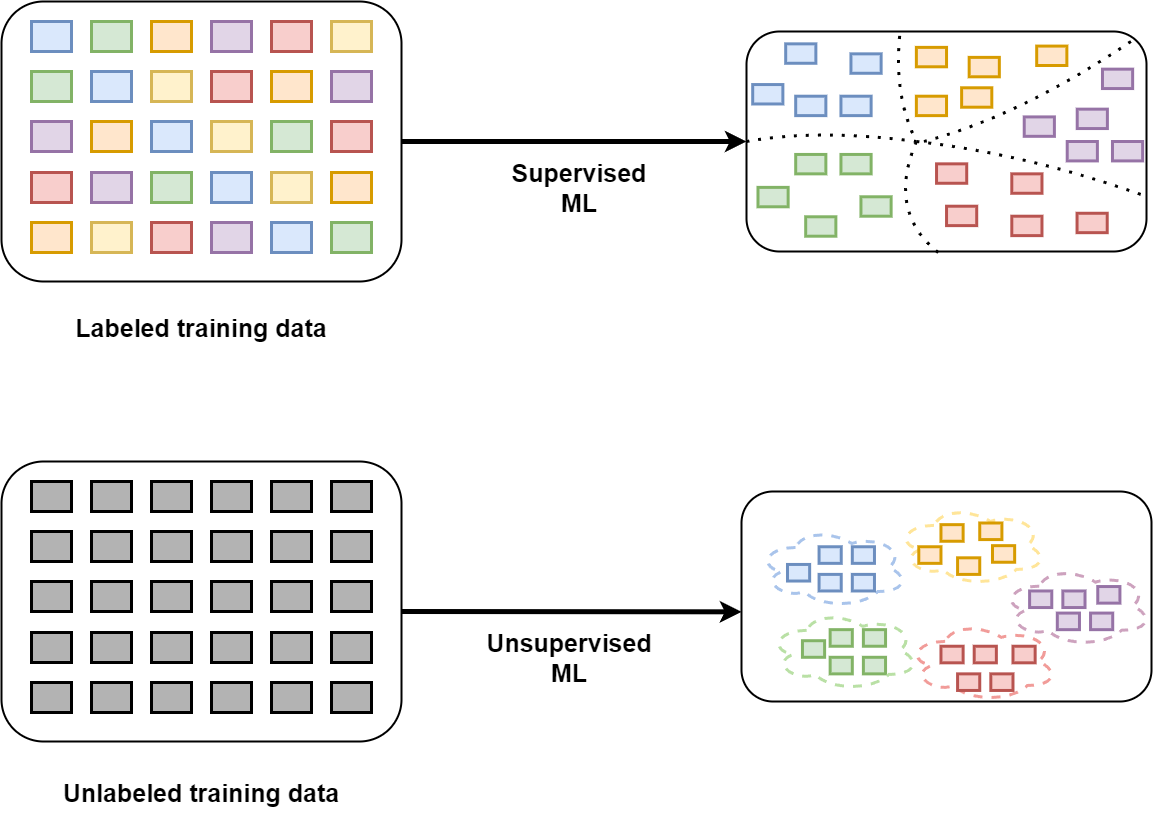
\includegraphics[width=.7\linewidth]{imgs/chapter_1/learning_paradigm.png}
    \caption{Machine learning paradigms}
    \label{fig:chap_1:ml_paradigms}
\end{figure*}

\subsubsection{Supervised learning}
\ac{SL} is the most fundamental and widely used learning paradigm. In SL, the training dataset $\mathcal{D}_{train} = \{(x_1, y_1), ..., (x_N,y_N)\}$ consists of a sufficient and representative amount of labeled samples (input-label pairs) that serve to learn a function $f_{\theta}$ approximating the true underlying relationship between $x_i$ and $y_i$.  
%that will determine the correct label for an unseen value $\tilde{x_i}$ and thus

The common SL tasks are classification tasks where we learn how to map the input $x_i$ to a discrete label (also category or class) and regression tasks where we map the input to a continuous value.

While effective for certain tasks, SL has notable limitations:
\begin{itemize}
    \item \textbf{Amount of labels}. SL requires a large amount of labeled data for training. However, the acquisition of these labels is often time-consuming and resource-intensive and may demand expert knowledge in domains such as networking or healthcare.
    \item \textbf{Label quality}. If the labels are erroneous, (which is possible since annotation process is done by humans), it can negatively impact the model performance.
    \item \textbf{Generalizability and overfitting}. SL models may require complex architectures to capture the underlying patterns in the training data. This complexity can lead to overfitting, causing poor performance on unseen data or data with different distribution.
    \item \textbf{Scalability}. The performance of SL improves with larger datasets. However, increasing the dataset size requires substantial computational resources and higher annotation costs, which may become impractical.
\end{itemize}


\subsubsection{Unsupervised learning}

\ac{UL} is a learning paradigm in which, unlike \ac{SL}, the learning process is conducted on unlabeled data. The model uncovers hidden patterns or relationships in the data without explicit guidance. UL can involve tasks such as discriminative, dimensionality reduction, or generative tasks. Generative UL focus on modeling the data distribution by learning a parametric approximation $p_{\theta}$ of the true data distribution $p$ enabling the generation of data samples $x_i \in \mathcal{D}$. Dimensionality reduction involves representing high-dimensional datasets in low-dimensional feature spaces while preserving intrinsic dataset properties. It is useful for tasks like noise reduction, data visualization, and reducing computational time and memory usage, especially before applying ML algorithms that struggle with high-dimensional data. Discriminative UL identifies relationships or boundaries between samples based on their similarities and differences. This can be achieved through clustering, which organizes samples into groups (clusters) based on these relationships, or through representation learning. Representation learning aims to construct feature extractors that identify the most meaningful and insightful representations from input data, enhancing downstream tasks and generalization to unseen data.


\subsubsection{Self-supervised learning}

\begin{figure*}[!ht]
    \centering
    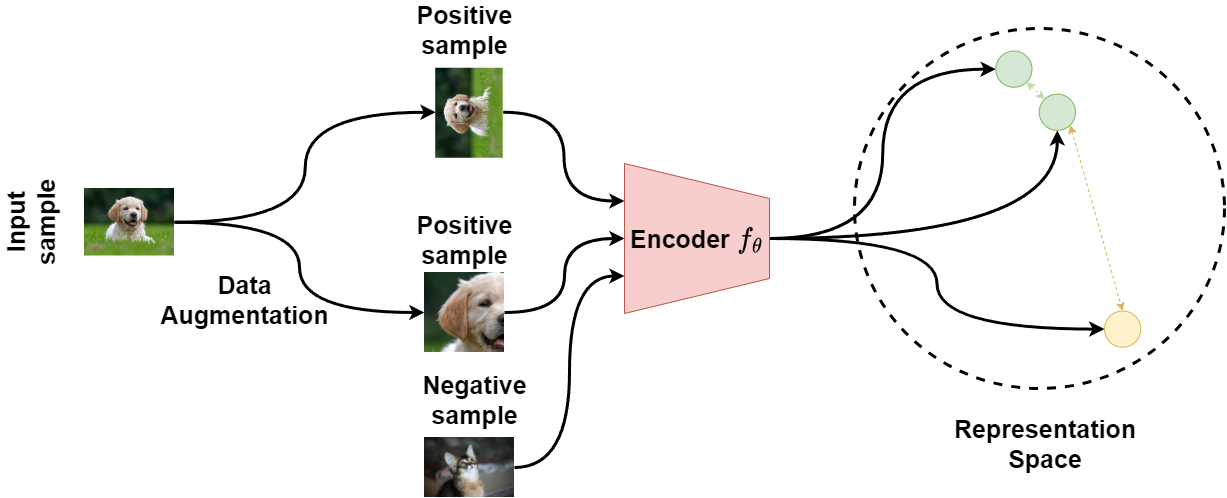
\includegraphics[width=.8\linewidth]{imgs/chapter_1/contrastive_learning.png}
    \caption{Contrastive learning}
    \label{fig:chap_1:contrastive_learning}
\end{figure*}

\ac{SSL}, a subset of UL, has gained immense popularity due to its remarkable performance across various tasks in \ac{NLP} and \ac{CV}. SSL leverages pseudo-labels derived from the inherent structure of unlabeled data to train models via pretext tasks. By solving these pretext tasks, the model generates self-supervision signals, enforcing it to learn task-agnostic features that capture essential patterns in the data (representation learning). Pretext tasks are designed based on the intended downstream tasks and typically include: i) \textbf{input completion} which consists in masking parts of the input and predicting the missing segments (e.g., predicting the next word in a sentence or reconstructing a portion of an image); ii) \textbf{transformation predictions} which consists in predicting transformations applied to the input (e.g., determining an image's rotation) or iii) \textbf{transformation invariance} which consists in learning invariant and meaningful features common across different representations of the same input after various transformations (e.g., using data augmentations).

Among SSL methods, \ac{CL} stands out as one of the most efficient and widely adopted frameworks. Its core idea, illustrated in Fig. \ref{fig:chap_1:contrastive_learning} involves training a feature extractor to cluster similar data (\textit{positive pairs}) in the feature space while pushing apart dissimilar data (\textit{negative pairs}). The key elements of CL include:
\begin{itemize}
    \item \textbf{Pair Selection:} Positive pairs and negative pairs are often generated using data augmentation. For example, in image classification, positive pairs can be created by applying different random crops or rotations to the same image, while negative pairs are generated by randomly selecting different images from the dataset.
    \item \textbf{Contrastive loss functions:} These include contrastive loss \cite{chopra2005learning}, triplet loss \cite{schroff2015facenet}, and InfoNCE loss \cite{oord2018representation}. The most commonly used is the \ac{NT-Xent} loss \cite{chen2020simple}. The most commonly used is \ac{NT-Xent} loss \cite{chen2020simple} which is defined as follows. 
    
    Given a mini-batch $\mathcal{B} = \{x_1, x_1^+, x_2, x_2^+, ..., x_N, x_N^+\}$ where $x_i^+$ is an augmented version of $x_i$, an encoder function $f_{\theta}$, NT-Xent loss will maximize the similarity between a representation of a sample $z_i = f_{\theta}(x_i)$ with its positive $z_i^+$ while minimizing its similarity with the $2N -2$ negatives $(z_j)_{\forall j \neq i \in \|1; N\|}$. The similarity is often measured with cosine similarity measure and the NT-Xent loss $\mathcal{L}_{NTXent}$ can be expressed as follows:

    \begin{equation}\label{eq:ntxent}
        \mathcal{L}_{NTXent} = - \frac{1}{2N} log \frac{exp(sim(z_i, z_i^+)/\tau)}{\sum_{k=1}^{2N} \mathbb{1}_{[k \neg i]} exp(sim(z_i, z_k)/\tau)}
    \end{equation}

    with $\tau$ a temperature hyperparameter that controls the relative importance of distance between pairs of points.
\end{itemize}

% Contrastive learning in general

% Contrastive learning on time series

\subsection{Training DL model}
Implementing a DL model involves a series of steps aimed at determining and optimizing the model's parameters by minimizing a loss function, ultimately achieving maximum performance on a given task. The process, summarized in Fig. \ref{fig:chap_1:dl_pipeline} is described as follows:
% Add figure of the pipeline


\begin{figure*}[!ht]
    \centering
    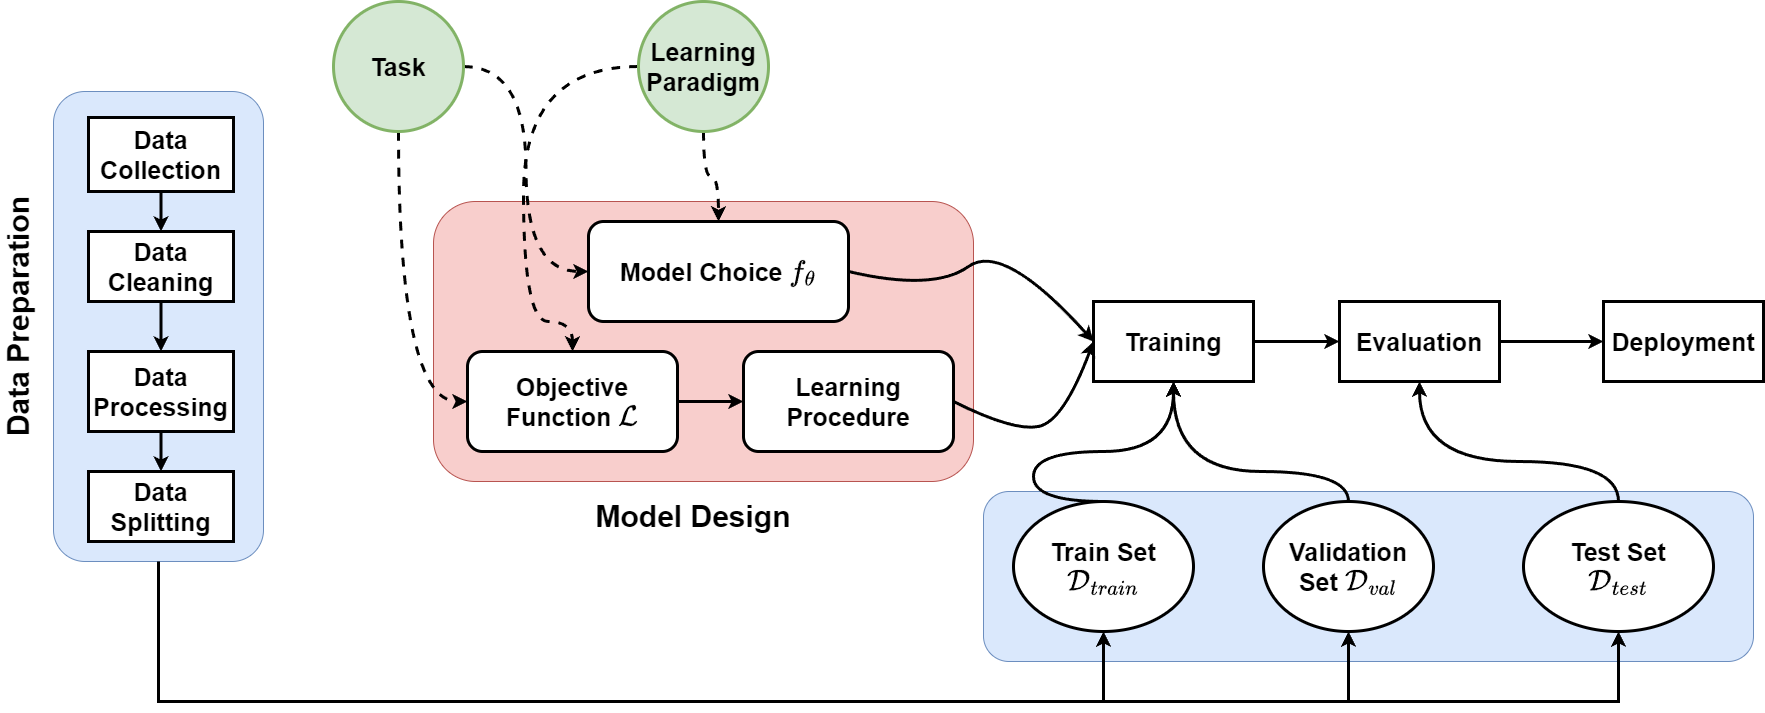
\includegraphics[width=.9\linewidth]{imgs/chapter_1/dl_pipeline.png}
    \caption{Deep learning implementation pipeline}
    \label{fig:chap_1:dl_pipeline}
\end{figure*}

\subsubsection{Dataset preparation}
The performance of a deep learning model is closely linked to the quality of the dataset. Preparing the dataset involves the following steps:

\begin{itemize}
    \item \textbf{Data collection :} Gather datasets that represent the problem domain. For this thesis, the focus is on time-series datasets for cloud gaming (CG) anomaly detection and virtual reality (VR) root-cause diagnosis.
    \item \textbf{Data cleaning :} Identify and remove missing, inconsistent or erroneous values in the dataset to ensure high-quality data.
    \item \textbf{Data processing :} Prepare data for model input through the following:
        \begin{itemize}
            \item Standardization/Normalization: Scale numerical features to a range (e.g., [0, 1]) or normalize them to have zero mean and unit variance.
            \item Categorical feature encoding: Apply one-hot or ordinal encoding for categorical features.
            \item Feature selection: Remove irrelevant or redundant features to improve learning efficiency. 
        \end{itemize}
    \item  \textbf{Data splitting :} the data should be split in three (03) sets. The training set used for the training of the model, the validation set to evaluate the model's performance during the training and the test set to assess the model's final performance and its generalizability.
\end{itemize}


\subsubsection{Design stage}
This stage involves selecting or defining the neural architecture ($f_{\theta}$) appropriate for the task and data type. To train the model, it is necessary to specify a loss function ($\mathcal{L}$), which quantifies the discrepancy between the model's outputs and the desired outputs (e.g., true labels in supervised learning). Common choices for the loss function include cross-entropy for classification tasks in supervised learning and reconstruction errors for autoencoders in unsupervised learning. The subsequent step is to choose an optimization technique to enhance the model's convergence speed and performance. The most widely used optimizers are \ac{SGD} and \ac{Adam}.


\subsubsection{Training stage}
The training stage is crucial as it aims to find the parameters that optimize task performance while ensuring generalizability. This involved solving an optimization problem that iteratively updates the model's parameters using only first-order derivatives. However, due to the large datasets typically used, calculating gradients across the entire dataset is impractical. Therefore, training is conducted using mini-batches (i.e., small subsets of training instances) and iterated over the entire dataset. The training process includes the following steps:
\begin{itemize}
    \item Sample a mini-batch $\mathcal{B} = {x_1, \ldots, x_{N_B}}$ from the training dataset.
    \item Perform a forward pass through the neural network to compute the outputs $f_{\theta}(x_i)$ for each sample ($x_i$) in the mini-batch.
    \item Calculate the average loss over all instances in the mini-batch: $\frac{1}{N_B} \sum_{i}^{N_B} \mathcal{L}(y_i, f_{\theta}(x_i))$.
    \item Compute gradients for model parameters with respect to the loss using backpropagation.
    \item Update the model parameters using an optimizer (e.g., SGD, Adam).
\end{itemize}


This setup is standard for supervised learning. For unsupervised or contrastive learning tasks, additional steps may be required. Hyperparameter tuning (e.g., learning rate, batch size, and number of epochs) is often necessary to enhance performance, alongside regularization techniques to mitigate overfitting.

\subsubsection{Evaluation stage and deployment}
After training, the model's performance is assessed on a test set using task-specific evaluation metrics. If the model demonstrates sufficient generalizability, it can be deployed in production environments. Post-deployment, it is essential to monitor the model's performance on new data to ensure continued effectiveness, and retraining may be necessary if performance declines.


%\takeaway{Deep learning (DL) leverages neural networks to design inference functions that solve tasks through various learning paradigms. Constructing a DL pipeline involves several key steps, which must be tailored to the specific task at hand. The goal is to create a model that is as generalizable as possible, ensuring its effectiveness when deployed in real-world applications.} % reformuler lien choix UL


% \takeaway{\ac{ML} and \ac{DL} have become essential for addressing complex problems across various domains. DL leverages neural networks, which excel in capturing intricate patterns, to design inference functions that solve tasks through various learning paradigms, including supervised, unsupervised, and self-supervised learning. Building a DL solution involves several key steps such as data preparation, model design, training, evaluation, and deployment, ensuring the performance and generalizability required for deployment in real-world scenarios.}


% \usage{In this thesis, we will follow this same DL implementation procedure, when designing ML solutions either for anomaly detection (Chapters \ref{chap:ml_evaluation}, , \ref{chap:cats}) or root-cause diagnosis (Chapter \ref{chap:diagnosis}).} % reformuler lien choix UL